% ============================================================================================================
\chapter{Distribution des effets entre ménages}\label{ch:distribution}
% ============================================================================================================

\section{De l'incidence fiscale au revenu réel}

La v0.7 mesurait les gagnants et les perdants sur les seuls prélèvements et prestations, aux revenus de l'année de
base. Le module M16 y ajoute, pour chaque ménage et à chaque horizon, les effets sur les salaires, l'emploi, les
revenus du patrimoine, les prix, l'indexation des pensions et prestations, et le coût des droits de succession
(chapitre~\ref{ch:equations}). Trois contrôles :
\begin{itemize}
\item \textbf{pas de double compte} : chaque composante du revenu n'est modifiée que par un canal ; la composante
fiscale des prix (TVA, taxe carbone) est retirée du déflateur, puisqu'elle est déjà dans le canal direct ;
\item \textbf{cohérence avec le modèle macroéconomique} : la somme des canaux (en valeur) est comparée à la variation du
revenu disponible des ménages du modèle macroéconomique, en termes réels et hors droits de succession (qui sont des
transferts en capital) ; l'écart résiduel est publié (colonne « résiduel » du tableau~\ref{tab:canaux}) : il est
inférieur à 0,3 point pour S2, S4 et S5, mais atteint 1,2 point pour S3 et 1,5 point pour S1 (la somme des canaux
micro y dépasse la variation macroéconomique ; l'écart n'a pas pu être attribué à un canal précis) ;
\item \textbf{avant la mise en œuvre} (2027), tous les écarts sont nuls (test automatisé).
\end{itemize}

\begin{limites}[Ce que M16 ne fait pas]
Les effets d'emploi sont calculés en espérance : un ménage dont un membre est au chômage reçoit la probabilité de
retour à l'emploi multipliée par le gain net, plutôt qu'un emploi ou rien. La part des ménages « gagnants » est donc
une part de ménages dont le revenu espéré augmente. Le patrimoine est approché par les revenus non salariaux et non
pensions du revenu fiscal (les patrimoines peu rémunérateurs, comme la résidence principale, ne sont pas vus), et les
droits de succession sont répartis selon cette assiette pondérée par l'âge (les héritiers effectifs ne sont pas
connus). Les salaires varient uniformément en pourcentage (sauf mesures propres au SMIC dans la microsimulation).
\end{limites}

\section{Résultats pour les stratégies}

{\tiny\setlength{\tabcolsep}{2.2pt}\begin{longtable}{llrrrrrrrrrr}\caption{Revenu disponible réel après propagation (M16), par décile de niveau de vie initial (\% du revenu), niveau de vie médian (\%), part des ménages gagnants / perdants (variation de plus de 0,5 \%), pauvreté (seuil fixe, points), Gini (×100). Ligne « statique » : incidence directe seule (v0.7).}\label{tab:distrib}\\ \toprule Stratégie & Année & D1 & D2 & D3 & D5 & D8 & D10 & Médiane & G / P & Pauvreté & Gini\\ \midrule\endfirsthead\toprule Stratégie & Année & D1 & D2 & D3 & D5 & D8 & D10 & Médiane & G / P & Pauvreté & Gini\\ \midrule\endhead
S1 Protection & 2030 & $+14{,}8$ & $+14{,}1$ & $+12{,}6$ & $+9{,}9$ & $+5{,}2$ & $+1{,}6$ & $+9{,}3$ & $84$ / $1$ & $-4{,}3$ & $-2{,}24$\\
 & 2035 & $+15{,}5$ & $+14{,}2$ & $+12{,}9$ & $+10{,}2$ & $+5{,}8$ & $+2{,}4$ & $+9{,}6$ & $93$ / $0$ & $-4{,}3$ & $-2{,}12$\\
 & 2047 & $+14{,}7$ & $+13{,}1$ & $+12{,}8$ & $+10{,}6$ & $+6{,}5$ & $+3{,}6$ & $+10{,}3$ & $99$ / $0$ & $-4{,}1$ & $-1{,}84$\\
 & statique & $+7{,}8$ & $+8{,}4$ & $+9{,}2$ & $+8{,}7$ & $+4{,}4$ & $+2{,}2$ & & & & \\
\addlinespace
S2 Emploi & 2030 & $-0{,}5$ & $+1{,}6$ & $+4{,}1$ & $+3{,}6$ & $+0{,}4$ & $-1{,}6$ & $+3{,}1$ & $41$ / $36$ & $-1{,}5$ & $-1{,}06$\\
 & 2035 & $-0{,}3$ & $+1{,}8$ & $+4{,}3$ & $+3{,}9$ & $+0{,}8$ & $-1{,}1$ & $+3{,}4$ & $53$ / $34$ & $-1{,}6$ & $-1{,}01$\\
 & 2047 & $-0{,}8$ & $+1{,}4$ & $+4{,}4$ & $+4{,}3$ & $+1{,}2$ & $-0{,}5$ & $+3{,}8$ & $61$ / $17$ & $-1{,}5$ & $-0{,}88$\\
 & statique & $-1{,}0$ & $+1{,}4$ & $+3{,}7$ & $+3{,}5$ & $+0{,}1$ & $-0{,}3$ & & & & \\
\addlinespace
S3 Productivité & 2030 & $+1{,}2$ & $+4{,}6$ & $+8{,}5$ & $+7{,}6$ & $+3{,}1$ & $+0{,}6$ & $+7{,}0$ & $62$ / $14$ & $-2{,}5$ & $-1{,}35$\\
 & 2035 & $+0{,}4$ & $+3{,}8$ & $+8{,}4$ & $+7{,}9$ & $+3{,}9$ & $+1{,}8$ & $+7{,}3$ & $64$ / $15$ & $-2{,}3$ & $-1{,}04$\\
 & 2047 & $-1{,}5$ & $+3{,}0$ & $+7{,}8$ & $+7{,}6$ & $+4{,}0$ & $+2{,}9$ & $+6{,}8$ & $60$ / $19$ & $-2{,}0$ & $-0{,}57$\\
 & statique & $-1{,}0$ & $+3{,}6$ & $+7{,}9$ & $+7{,}7$ & $+2{,}9$ & $+1{,}6$ & & & & \\
\addlinespace
S4 Redressement & 2030 & $-4{,}5$ & $-4{,}1$ & $-2{,}5$ & $-1{,}6$ & $-1{,}4$ & $-2{,}9$ & $-1{,}5$ & $0$ / $97$ & $+1{,}2$ & $-0{,}07$\\
 & 2035 & $-4{,}8$ & $-4{,}3$ & $-2{,}7$ & $-1{,}8$ & $-1{,}6$ & $-3{,}2$ & $-1{,}7$ & $0$ / $99$ & $+1{,}3$ & $-0{,}10$\\
 & 2047 & $-4{,}5$ & $-4{,}0$ & $-2{,}7$ & $-1{,}9$ & $-1{,}8$ & $-3{,}4$ & $-1{,}9$ & $0$ / $100$ & $+1{,}3$ & $-0{,}15$\\
 & statique & $-1{,}5$ & $-1{,}0$ & $-1{,}0$ & $-0{,}9$ & $-0{,}9$ & $-0{,}5$ & & & & \\
\addlinespace
S5 Global & 2030 & $-2{,}0$ & $-0{,}1$ & $+2{,}5$ & $+2{,}4$ & $-0{,}0$ & $-2{,}3$ & $+2{,}0$ & $34$ / $30$ & $-0{,}9$ & $-0{,}86$\\
 & 2035 & $-2{,}3$ & $-0{,}2$ & $+2{,}5$ & $+2{,}4$ & $-0{,}1$ & $-2{,}3$ & $+2{,}0$ & $34$ / $44$ & $-0{,}9$ & $-0{,}87$\\
 & 2047 & $-2{,}2$ & $-0{,}1$ & $+2{,}4$ & $+2{,}3$ & $-0{,}2$ & $-2{,}6$ & $+1{,}9$ & $33$ / $47$ & $-0{,}9$ & $-0{,}92$\\
 & statique & $-0{,}4$ & $+1{,}5$ & $+3{,}1$ & $+2{,}7$ & $-0{,}1$ & $-0{,}3$ & & & & \\
\addlinespace
A (v0.6) & 2030 & $-0{,}4$ & $+0{,}2$ & $+1{,}0$ & $-0{,}0$ & $-2{,}1$ & $-3{,}9$ & $-0{,}6$ & $22$ / $73$ & $-0{,}5$ & $-1{,}00$\\
 & 2035 & $-0{,}6$ & $+0{,}0$ & $+0{,}8$ & $-0{,}2$ & $-2{,}3$ & $-4{,}2$ & $-0{,}8$ & $21$ / $74$ & $-0{,}5$ & $-1{,}02$\\
 & 2047 & $-0{,}8$ & $-0{,}1$ & $+0{,}7$ & $-0{,}3$ & $-2{,}5$ & $-4{,}4$ & $-0{,}8$ & $21$ / $74$ & $-0{,}4$ & $-1{,}03$\\
 & statique & $-2{,}6$ & $-0{,}9$ & $+0{,}7$ & $+0{,}4$ & $-1{,}8$ & $-1{,}8$ & & & & \\
\addlinespace
B (v0.6) & 2030 & $-4{,}0$ & $-3{,}8$ & $-2{,}2$ & $-1{,}8$ & $-1{,}9$ & $-3{,}1$ & $-1{,}9$ & $7$ / $80$ & $+1{,}1$ & $-0{,}14$\\
 & 2035 & $-5{,}2$ & $-4{,}2$ & $-2{,}3$ & $-1{,}6$ & $-1{,}5$ & $-2{,}2$ & $-1{,}7$ & $11$ / $78$ & $+1{,}2$ & $+0{,}08$\\
 & 2047 & $-7{,}3$ & $-5{,}2$ & $-2{,}9$ & $-1{,}7$ & $-1{,}2$ & $-0{,}9$ & $-2{,}0$ & $10$ / $82$ & $+1{,}6$ & $+0{,}60$\\
 & statique & $-1{,}8$ & $-1{,}3$ & $-0{,}8$ & $-0{,}9$ & $-1{,}4$ & $-1{,}3$ & & & & \\
\addlinespace
C (v0.6) & 2030 & $+9{,}2$ & $+5{,}3$ & $+4{,}2$ & $+3{,}5$ & $+1{,}3$ & $-3{,}4$ & $+3{,}1$ & $63$ / $12$ & $-1{,}9$ & $-1{,}75$\\
 & 2035 & $+9{,}1$ & $+5{,}2$ & $+4{,}1$ & $+3{,}4$ & $+1{,}5$ & $-2{,}9$ & $+3{,}0$ & $61$ / $16$ & $-1{,}8$ & $-1{,}61$\\
 & 2047 & $+7{,}4$ & $+4{,}2$ & $+3{,}1$ & $+2{,}7$ & $+1{,}2$ & $-2{,}5$ & $+2{,}0$ & $46$ / $32$ & $-1{,}3$ & $-1{,}21$\\
 & statique & $+11{,}3$ & $+7{,}7$ & $+5{,}1$ & $+4{,}2$ & $+1{,}7$ & $-1{,}3$ & & & & \\
\addlinespace
D (v0.6) & 2030 & $-4{,}7$ & $-4{,}0$ & $-2{,}9$ & $-4{,}2$ & $-6{,}6$ & $-11{,}0$ & $-4{,}9$ & $8$ / $89$ & $+1{,}1$ & $-1{,}65$\\
 & 2035 & $-6{,}4$ & $-4{,}8$ & $-3{,}4$ & $-4{,}5$ & $-7{,}1$ & $-11{,}6$ & $-5{,}2$ & $6$ / $90$ & $+1{,}4$ & $-1{,}67$\\
 & 2047 & $-7{,}1$ & $-5{,}2$ & $-3{,}6$ & $-4{,}5$ & $-7{,}2$ & $-11{,}9$ & $-5{,}2$ & $6$ / $90$ & $+1{,}5$ & $-1{,}71$\\
 & statique & $-3{,}6$ & $-1{,}7$ & $-0{,}8$ & $-1{,}9$ & $-4{,}7$ & $-6{,}4$ & & & & \\
\addlinespace
R (v0.6) & 2030 & $+9{,}7$ & $+4{,}7$ & $+2{,}1$ & $+0{,}9$ & $-1{,}3$ & $-6{,}0$ & $+0{,}4$ & $39$ / $54$ & $-1{,}1$ & $-1{,}98$\\
 & 2035 & $+9{,}3$ & $+4{,}5$ & $+1{,}8$ & $+0{,}7$ & $-1{,}4$ & $-5{,}9$ & $+0{,}1$ & $40$ / $55$ & $-0{,}9$ & $-1{,}87$\\
 & 2047 & $+8{,}4$ & $+4{,}1$ & $+1{,}5$ & $+0{,}6$ & $-1{,}4$ & $-5{,}7$ & $-0{,}0$ & $39$ / $56$ & $-0{,}7$ & $-1{,}75$\\
 & statique & $+8{,}7$ & $+4{,}4$ & $+1{,}7$ & $+1{,}0$ & $-1{,}3$ & $-4{,}0$ & & & & \\\bottomrule\end{longtable}}

\begin{figure}[htbp]\centering
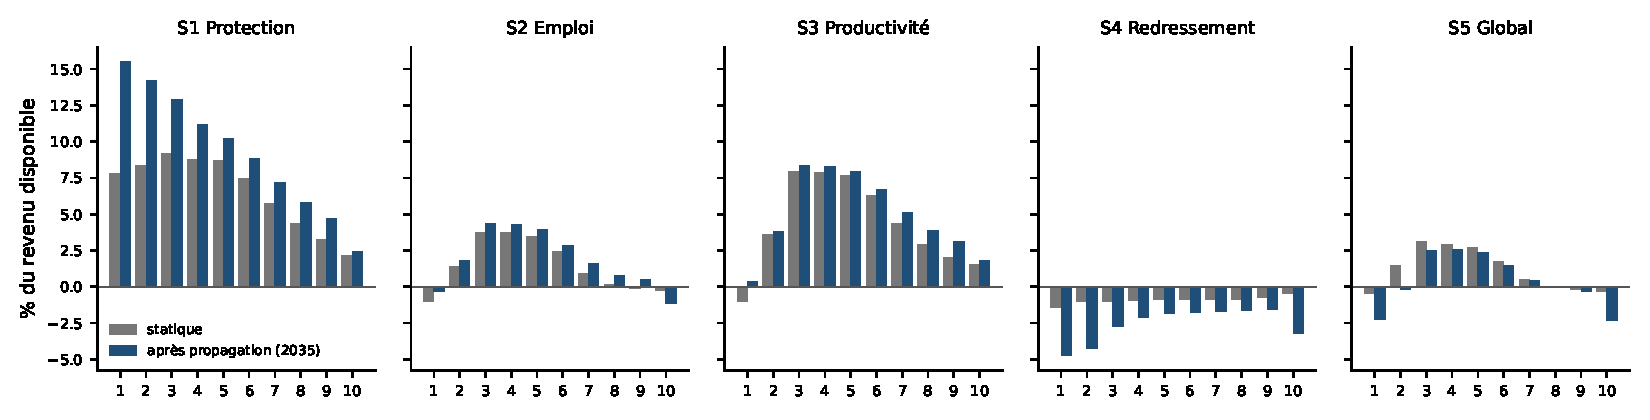
\includegraphics[width=\linewidth]{deciles_dynamique.pdf}
\caption{Variation du revenu disponible par décile : incidence directe seule (gris, méthode de la v0.7) et revenu réel
après propagation en 2035 (bleu).}\label{fig:dec_dyn}
\end{figure}

\begin{table}[htbp]\centering\scriptsize
\caption{Contribution des canaux à la variation du revenu disponible réel moyen en 2035 (\% du revenu) et résiduel de
cohérence avec le modèle macroéconomique.}\label{tab:canaux}
\tabfit{../tables/distribution_canaux.tex}
\end{table}

\paragraph{Ce qui change par rapport à l'incidence directe.}
\begin{itemize}
\item \textbf{Les prélèvements sur les entreprises et les patrimoines ont désormais des perdants.} Toutes les stratégies
augmentent de 50 \% les droits de succession : le dernier décile supporte un coût d'environ 1 300 € par unité de
consommation et par an. Avec la hausse de l'IS (S1, S4, S5), il perd aussi par les salaires (incidence) et les revenus
du patrimoine. Dans S5, le dernier décile perd 2,3 \% de revenu réel en 2035, alors qu'il perdait 0,3 \% en incidence
directe.
\item \textbf{La baisse des allocations chômage fait des perdants parmi les plus modestes} : elle figure dans S2, S3, S4
et S5 ($-25$ \%) et coûte de 700 à 1 600 € par unité de consommation aux ménages dont la personne de référence est au
chômage. Dans S2 et S5, le premier décile perd (de 0,3 \% et 2,3 \% en 2035) ; dans S3, le canal emploi (245 € par unité
de consommation) compense à peine la perte directe.
\item \textbf{Le canal de l'emploi profite d'abord aux deux premiers déciles} dans S1 et S2 (retours à l'emploi de
chômeurs et d'inactifs : 200 à 400 € par unité de consommation en 2035). Dans S3, il profite surtout au dernier décile
(800 €), parce que le maintien en emploi des seniors (âge légal) concerne des ménages aux salaires élevés.
\item \textbf{Les prix et l'indexation reprennent une partie des gains} : dans S1, la hausse des salaires et la baisse du
chômage font monter les prix ; le canal « prix » retire 3,3 points de revenu réel moyen en 2035.
\item \textbf{S4 fait perdre tous les déciles} de 1,6 à 4,8 \% du revenu réel en 2035, le premier et le dernier décile
davantage (allocations chômage pour le premier ; successions, IS, salaires pour le dernier). Les chômeurs perdent 9 \%,
les indépendants 3,2 \%, les retraités et les salariés 1,9 \%. La pauvreté augmente de 1,4 point.
\item \textbf{S1 est la seule stratégie sans perdants} (93 \% de ménages gagnants, aucun perdant de plus de 0,5 \%) ;
la pauvreté baisse de 4,3 points.
\end{itemize}

\paragraph{Par statut, logement et famille (2035).} Dans S1 et S3, les familles monoparentales, les familles
nombreuses, les locataires (surtout en HLM) et les moins de 45 ans gagnent le plus ; les propriétaires et les retraités
le moins. Dans S2, S3, S4 et S5, les ménages dont la personne de référence est au chômage perdent (de 4 à 9 \%). Les
tableaux suivants donnent les montants en € par unité de consommation (et en \% du revenu).

\begin{table}[htbp]\centering\scriptsize
\caption{Revenu réel après propagation par statut de la personne de référence, 2035 (€ par UC et \%).}
\tabfit{../tables/distribution_statut.tex}
\end{table}

\begin{table}[htbp]\centering\scriptsize
\caption{Par statut d'occupation du logement, 2035.}
\tabfit{../tables/distribution_occupation.tex}
\end{table}

\begin{table}[htbp]\centering\scriptsize
\caption{Par configuration familiale, 2035.}
\tabfit{../tables/distribution_famille.tex}
\end{table}

\begin{table}[htbp]\centering\scriptsize
\caption{Par âge de la personne de référence (transferts entre générations), 2035.}
\tabfit{../tables/distribution_age.tex}
\end{table}

\paragraph{Générations.} Les stratégies qui augmentent les prestations liées à l'activité (S1, S2, S3, S5) transfèrent
du revenu vers les ménages de moins de 45 ans ; les plus de 60 ans gagnent peu (S1, S3) ou perdent (S2, S5, S4). Dans
S3, le relèvement de l'âge légal à 66 ans est mesuré en revenu : les ménages proches de l'âge légal qui travaillent
gagnent un salaire, ceux qui perçoivent une pension la perdent pendant la durée du report ; le temps de retraite perdu
n'est pas valorisé.

\begin{encadre}{Trois défauts de la distribution dynamique corrigés pendant la phase 3.1}
La réoptimisation (chapitre~\ref{ch:optimisation}) a fait apparaître un résultat suspect : relever l'âge légal à 65 ans
augmentait le niveau de vie du premier décile de 9 \% en 2047. Les actifs seniors supplémentaires étaient traités comme
des inactifs d'âge actif entrant sur le marché du travail, concentrés dans le bas de la distribution. Ils sont désormais
attribués aux ménages proches de l'âge légal (pseudo-cohorte : salaire maintenu, allocation chômage, pension non
versée) : le premier décile perd 1 \% en 2047. Deuxième défaut : la baisse des allocations chômage, les transferts aux
ménages et le point d'indice, absents de la microsimulation, n'avaient ni gagnants ni perdants directs ; ils sont
répartis par des clés explicites (nombre de chômeurs, prestations, salaires). Troisième défaut : le contrôle de
cohérence comparait un revenu nominal macroéconomique, qui ne contient pas la TVA, à une somme microéconomique qui la
contient ; il est fait en termes réels. Toutes les simulations ont été relancées. La principale conséquence est que la
baisse de 25 \% des allocations chômage, présente dans quatre stratégies sur cinq, fait désormais apparaître des
perdants dans le premier décile.
\end{encadre}
